\chapter{Логово Змия}

Хвойка шутил, что своими лёгкими он высушил весь музей – Киевский городской музей древностей, сейчас там Национальный художественный музей Украины. Шутил так потому, что стоял у истоков его создания, провел там много времени и оттого, мол, заболел туберкулезом.

Но дом Хвойки на Кирилловской площади, с которой виднелся Смородинский спуск, наводит на другую мысль. Может быть много, ой много времени провел Хвойка в сырых пещерах Кирилловских высот, где в самой глубине воздух плотный от осыпающейся суглинной пыли. Она покрывает тебя всего тонким шероховатым налетом и заставляет кашлять.

Хвойка скрупулезно отметил на карте все здешние пещеры? Где же описание их исследований? А помните, как члены киевского отдела Императорского военно-исторического общества Стеллецкий, Дитрихс, профессор Завитневич хотели раскапывать пещеру к северной стены Кирилловской церкви, да Хвойка не явился, и без него не стали? Обошел подробное описание пещер Смородинского спуска и Антонович, сделав упор, как увидим далее, на куче доисторического мусора у входа в главную из них.

По былинам и сказаниям, мы приблизительно вычислили место обитания «змеев» – Кирилловские высоты, цепь холмов над улицей Кирилловской. Но здесь было много пещер, не только на Смородинском спуске. Нет однозначного ответа, какая пещера является «той самой», логовом Змия, или Кирилловской пещерой. По былинам, змей обитал во множестве пещер. В наше время логовом Змия считают одну пещеру на Смородинском спуске. По непрерывному изустному преданию ли, между людьми передающемуся? Или некий краевед, отыскав подземелье сие, соотнес его с логовом? Неведомо.

А какие «более 20 пещер», как пишут в книжках по археологии, исследовал профессор Антонович? На Смородинском спуске ли? Да, на это Антонович указывает в работе «Киев в дохристианское время»\cite{antpublect01}:

\begin{quotation}
Так как группа этих пещер прилегает к месту, обследованному г. Хвойко, и так как предметы, находимые в обоих случаях, тождественны, то это заставляет предполагать, что стоянки служили, быть может, летними жилищами, обитатели которых на зиму перебирались в пещеры.
\end{quotation}

Хвойка исследовал окрестности Кирилловской стоянки, включая усадьбу Светославского, а последняя близка к Смородинскому спуску. Описанная Антоновичем уцелевшая на Смородинском спуске пещера имеет вид спирали, как и Логово Змиево. Поскольку остальные пещеры были где-то рядом, значит, все они находились на Смородинском спуске. К сожалению, Антонович нигде не называет исследованную им пещеру Кирилловской, а это упростило бы дело, ибо в источниках пещера Антоновича не привязана к Кирилловской.

Но раз знаменитая пещера на всю округу только одна, можно с большой вероятностью предположить, что Кирилловская и Антоновича тождественны.

Кроме статей Антоновича, существует еще одна, малоизвестная, доктора естественных наук, ботаника, геолога, палеонтолога и минеролога Афанасия Семеновича Роговича (1812-1878), «Об экскурсии, произведенной в 1875 г. по предложению Киевского общества естествоиспытателей», напечатанная в «Записках киевского общества естествоиспытателей» (1876, том IV, выпуск 3). Статья описывает местность шире, посему начнем с нее. 

Пещерам уделена только часть статьи. Разберем ее подробно. Незначительное буду выпускать.

\begin{quotation}
Об относительной древности пещер близ Кириловского монастыря\\

Искусственные пещеры в здешнем крае и в западной Европе остаются до сих пор мало исследованными. [...] Об некоторых из них существуют легенды: так например о змеиной пещере близ Кирилловского монастыря и пещере Лысой горы.
\end{quotation}

Судя по сказанному несколько далее, под Лысой горой имеется в виду Лысая гора на Кирилловских высотах. Предание про нее Рогович умалчивает, и нигде более о ней я не читал.

\begin{quotation}
Пещеры в здешнем крае встречаются или отдельными, как например межигорская пещера, китаевская пещера, пещера на Лысой горе, чигиринская пещера, полтавская, гадячская черниговская, или группами, состоящими из нескольких пещер, как пещеры близ Кириловского монастыря и в Гадючьем яру, недалеко от Киева.

Большею частью пещеры расположены в лесистых оврагах, вблизи источников ключевой воды и имеют вид длинных, простых или ветвистых коридоров, выкопанных в горах, покатых с двух сторон, для вырытия в них двух выходов с одной и другой стороны, что необходимо для вентиляции и защиты или имеют винтообразную форму в два оборота, составляющих верхний и нижний этажи с одним верхним входом.
\end{quotation}

Винтообразные пещеры не правило, а скорее особенность Змиевой пещеры на Смородинском спуске. Судя по статье Роговича, не одна эта пещера здесь имела подобное строение, а несколько.

\begin{quotation}
В прошедшем 1875 г. мне удалось только некоторые из них исследовать на Загоровщине в овраге Балашова, близ Кириловского монастыря и по найденным в них остаткам и изделиям человека определить относительную древность. 
\end{quotation}

Отсюда мы можем сделать несколько выводов. Загоровщиной слыла не только местность с пещерами из дела Бейлиса, но и Смородинский спуск. Овраг последнего назывался оврагом Балашова. Майор по фамилии Балаш прежде владел здесь участком земли. Владелица на 1875 год – дочь майора, Елизавета Балаш. Земля граничила с участком Баггавутов, что лежал ближе к Репяхову яру, условно говоря по Врубелевский спуск.

\begin{quotation}
При этом своим долгом считают выразить мою живейшую благодарность их превосходительствам Александру Федоровичу и Елизавете Дмитриевне Багговутам, занимающимся раскопками этих пещер в продолжении нескольких лет, за содействие в моих исследованиях и доставление кремневого серпа и нескольких других предметов, в них найденных.
\end{quotation}

Получается, что хотя нынешним Смородинским спуском владели Балаши, семья Багговутов вовсю занималась там раскопками.

\begin{quotation}
В начале упомянутого оврага находится глубокая вертикальная четыреугольная яма, открытая с восточной стороны, с этой же стороны несколько уступов для входа внутрь ея; стены ея тщательно выровнены и отшлифованы.
\end{quotation}

Невозможно сопоставить эту яму с современной местностью, и неясно, как понимать «начало оврага» – самый верх его или самый низ.

\begin{quotation}
Вблизи этой ямы отрыт скелет человека, большого роста; из него доставлена мне была А. Ф. Багговутом голова монгольского племени пробитая щупом насквозь, что имеет вид раны, сделанной огнестрельным оружием. Голова эта отличается значительною величиною, плоским лбом, выпуклыми надбровными дугами, очень развитыми темяными широкими скуловыми костями; в верхней и нижней челюстях с каждой стороны находятся по четыре коренных зуба, что означает молодой возраст, окрашенных черным цветом, заметно сохранившихся.
\end{quotation}

Большой череп и выпуклые надбровные дуги подходят скорее неандертальцу, нежели монголоиду. Однако, у неандертальцев лоб – покатый и с эдакой горкой.

Сомневаюсь, что голову можно пробить насквозь щупом и допускаю, что в самом деле, в древности, произошло убийство из огнестрельного оружия.

\begin{quotation}
При спуске с горы отрыты две круглые вертикальные ямы, имеющие вид глубоких колодцев, с остатками очень длинных лестниц. Эти ямы на половине их глубины соединяются горизонтальною пещерою, вышиною в рост человека.
\end{quotation}

«При спуске с горы» – сходя с нее вниз, или же у подножия, либо около некой дороги, буквально при спуске с горы? А из чего сделаны лестницы? 

\begin{quotation}
Как на дне ям, так и около их отверстия найдены слои ракушек Unio pictorum и Anadonta anatica, называемых скойками и употребляемых до сих пор в некоторых деревнях Херсонской губернии в пищу. Эти ракушки были перемешаны с рыбными костями и черепками глиняной посуды черного цвета, грубо сделанных без гончарного станка и содержащими крупные зерна кварца.

Слои ракушек без всякого сомнения составляют кухонные остатки первобытного человека; такие же остатки находятся недалеко от этих пещер, на так называемом езуитском погребку и на Лысой горе, где они имеют вид отдельных сорных куч.
\end{quotation}

Здесь отмечается близость к оврагу Балашова Лысой горы и некоего езуитского погребка. Значит, Лысая гора со своей пещерой – та, что слывет ныне Юрковицей. Про езуитский погребок ничего не ведаю.

\begin{quotation}
По спуску к Кириловской улице находится целый ряд пещер, идущих почти параллельно от севера на юг.
\end{quotation}

Речь однозначно идет о пещерах на западном склоне оврага Балашова, Смородинского спуска. Он имеет явно выраженное направление с севера на юг. В 21 веке на этом склоне доступен вход лишь в одну давнюю пещеру – Змиева, да в две «малые».

\begin{quotation}
Вход в эти пещеры состоит из уступов, в некоторых из них на расстоянии от входа при стенке сложены булыжники, часто пережженные и смешанные с черепками глиняной посуды грубой работы, кусками прокаленной глины, углями, золою и ракушками.
\end{quotation}

Итак, Рогович как и Бобровский говорит об уступах при входах в пещеры.

\begin{quotation}
В одной из пещер против сложенных булыжников находится отверстие для прохода дыма и закоптевшая стена. 

Эти места без сомнения служили очагами для пещерных обителей. Там же нередко встречаются разбитые бычачьи и лошадиные кости.

В одной из винтообразных пещер, длиною в двадцать пять саженей, по обоим сторонам главного коридора  находится по две небольшие камеры, имеющие вид конур; вход в них круглый, чрез который может пролезть один человек.
\end{quotation}

Из последнего могу предположить, что кроме Змиевой, тут были и другие пещеры в виде винта.

\begin{quotation}
Кроме того в них найдены: обточенный в виде конуса кусок красного песчаника, который, вероятно, употреблялся для раскалывания и раздробления костей, белый шарик, сделанный из мелкого известкового камня, составлявший голову шпильки и конечный обломок кремневого орудия, имеющего вид серпа, с выпуклой стороны острого и на вогнутой стороне правильно зазубренного.

Пещера, в которой найдены означенные пре\-дметы, недалеко от входа в верхний этаж имела очаг, сложенный из булыжников, смешанных с черепками грубой глиняной посуды, костями быка и двустворчатыми пресноводными ракушками, какие и в настоящее время  водятся в Днепре, отверстие для выхода дыма и закопченную стену;
\end{quotation}

Припомним это, когда станем разбирать статью Антоновича – кажется, речь идет об одной и той же пещере, Змиевой. Удивительно, что оба ученых молчат о внутреннем содержимом пещер, о граффити на стенах – вообще о том, что могло отличать в описании одну пещеру от другой. 

\begin{quotation}
в нижнем конце пещеры слышен постоянный гул подобный тому, который слышен в винтообразной одностворчатой раковине который зависит от вентиляции.
\end{quotation}

Когда я долез до последней комнатки Змиевой пещеры, за узким коридором-шкурником, то не слышал в нем ничего подобного.

\begin{quotation}
Подобные пещеры в большом количестве находятся на трех возвышенных местах, разделенных оврагами. 
\end{quotation}

Это общее утверждение, сходное с «двадцатью пещерами» найденными тут Антоновичем, даже еще более общее. Ибо если принять на веру «подобие» пещер, то следует принять, что от Смородинского спуска до автобазы, до «пещер из дела Бейлиса» (а именно так можно толковать «три возвышенных места, разделенных оврагами»), было именно множество удивительных, тысячелетних винтообразных больших протяженностью пещер с низенькими потолками. Так это или нет, все ли здешние пещеры были подобны Змиевой по размеру и строению, уцелела и доступна к посещению только одна – Змиева, она же Кирилловская.

\begin{quotation}
Судя по найденным в них означенным предметам можно предположить, что они составляли жилища первой половины каменного периода первобытного человека, раньше свайных построек.
\end{quotation}

Однако речь и у Роговича, и у Антоновича идет про обжитость предбанников в пещеры, обжитость древними людьми. Ничего не говорится про глубины пещер.

\begin{quotation}
А. Ф. Багговут сообщил мне также, что в пещерах найдены были две человеческие головы обыкновенной величины, сделанные грубо из красного камня и доска из красного шифера, но к сожалению эти предметы, имеющие важный научный интерес, мне до сих пор еще не доставлены.
\end{quotation}

Я не слышал о подобных археологических находках где-либо еще и конечно понимаю сожаление Роговича. Любопытно, что еще отыскали супруги Багговуты и не поделились этим с общественностью? Никто не раскапывал здешнюю местность более, чем они.

\begin{quotation}
На поляне вблизи Кириловской улицы найдено двенадцать обезглавленных скелетов, расположенных в круге, головы от них погребены были в другом месте, в кургане. Об этих скелетах в народе существует темное предание.
\end{quotation}

Где именно была эта поляна, что за предание? В явно обрядовом положении скелетов угадывается солнце, на обрядовость указывает и число – дюжина. 

\begin{quotation}
Грунт земли Кириловской улицы и вообще Подола нанеcен с гор и течением Днепра после вырытия пещер, что видно из слоев земли, обнажаемых при копании рвов под постройки, останкам животных и изделиям человека.

В том месте где находятся древние остатки монастыря Иоанна Богослова, недалеко Иорданской церкви в усадьбе Марра, при копании рва, на глубине более двух саженей в желтой глине обнажился слой раковин, тех же самых видов, которые и в настоящее время водятся в Днепре;
\end{quotation}

Здесь мы начинаем знакомиться с новыми подробностями раскопок в усадьбе Марр. Про раскопки мы уже читали в статье Антоновича 1877 года «О древнем кладбище у Иорданской церкви в Киеве». Но вот что сообщает Рогович: 

\begin{quotation}
в верхнем черноземном слое толщиною до полутора сажени, в нижней его части найдена печь для сожигания покойников, горшки с посмертным пеплом и уцелевшими полуобгоревшими костями человеческими, серьги из серебряной проволоки с надетыми на нее одною или тремя разноцветными бусами, одна сережка из золотой проволоки, серебряная куфическая монета с приделанным ушком для ношения на шее; 

над языческим кладбищем, на незначительной глубине находятся остатки татарского побоища: множество черепов татарских и славянских перемешаны между собою и похоронены без всякого порядка\footnote{Не об этом ли месте говорил Антонович касательно останков 4000 человек?}; 

в одной из могил найдено три скелета человеческих вместе с скелетом лошади, седло с стременами. Голова всадника и лошади раздроблены кистенем, круглым булыжником, зашитым в кожу, найденным вблизи скелетов; в той же яме найдены большой железный меч, копье, верхняя часть железного шлема, имеющая вид чашки, два тонких серебряных креста, сумка с железными стрелами, небольшой брусок, вероятно, употреблявшийся для точения стрел, часть пояса и две больших вызолоченных медных пряжки с выпуклыми украшениями, из которых наибольшее имеет вид великокняжеской шапки, игла из красной меди и железный бердыш.
\end{quotation}

У Антоновича мы не узнали про печи для сожжения останков, и про следы явно ритуального убийства всадника с лошадью тут же вероятно над могилой. Но про Смородинский спуск у Роговича более ничего нет.

Обратимся к другой статье, тоже Антоновича. Судя по датам, он исследовал окрестности и пещеру годом позже Роговича (и сообща с ним), в 1876-м. Оба были знакомы, ведь Рогович был профессором в том же университете святого Владимира, где преподавал и Антонович, правда в указанное время Рогович, с 1868 года, находился в отставке, а в 1878 году умер.

Открываем сборник «Чтения в историческом обществе Нестора летописца. Книга 1. 1873-1877»\cite{chtenianestora01} и читаем статью со страницы 244, «Археологические находки и раскопки в Киеве и в Киевской губернии в течении 1876 года». Именно эта статья Антоновича является основным источником письменных сведений о пещере и неоднократно пересказана позднейшими учеными:

\begin{quotation}
самая многочисленная группа известных мне пещер находится у Кирилловского монастыря. Возвышенность, на которой расположен монастырь, отделяется от другой возвышенности, прилегающей к ней с южной стороны, глубоким ветвистым оврагом, на склонах которого, на различной высоте, расположены пещеры.

Многие из них были расчищены от наноса в последнее время, благодаря случайному обстоятельству: у окрестных жителей существует неясное предание о том, что в данной местности будто спрятан был в землю гетманом Мазепою большой клад; увлекаясь этим преданием и замечая на обрывистых берегах оврага отверстия пещер, кладоискатели сочли их коридорами, ведущими к погребам Мазепы, и, не жалея трудов и издержек, принялись расчищать пещерные ходы от наполнявшего их землистого наноса\footnote{Не супруги Багговуты ли эти местные жители, о коих пишет Антонович?}. 

Конечно, ни погреба, ни клада в конце каждого пещерного хода не оказалось, но, при расчистке, вместе с наносом, рабочие выбросили из пещер и те драгоценные в научном отношении, но не представлявшие для них интереса, бытовые остатки, которые свидетельствовали об условиях жизни древних пещерных обитателей
\end{quotation}

Прервем чтение – продолжим его позже. Антонович в «Киев в дохристианское время» сообщает подробности – а речь идет именно о заинтересовавшей его группе пещер, примыкающей к местам, что исследовал Хвойка: 

\begin{quotation}
так, многие пещеры из группы, расположенной у Кирилловского заведения, были совершенно испорчены для науки вследствие недоразумения; именно одна из владелиц усадьбы, увлекшись слухами о кладах, спрятанных будто бы Мазепой в подвалах этой местности, стала расчищать лессовые пещеры до дна, причем все остатки каменного века были выброшены; только одну из них удалось исследовать раньше этой расчистки, и она оказалась, несомненно, жилищем людей каменного века.
\end{quotation}

Итак, эти пещеры Антонович относит к «группе, расположенной у Кирилловского заведения». Стало быть, речь не идет о пещерах, затерянных в Репяховом яру. Владимир Бонифатьевич определенно подразумевает пещеры Смородинского спуска. На это уже можно положиться в рассуждениях.

Ведь например неясно, что имеет в виду Сементовский в своей книге\cite{sement01}, помещая короткий раздел «Кирилловская пещера»:

\begin{quotation}
Находится на оной стороне холма, покрытого деревьями. Пещера эта устройством подобна лаврским пещерам. Предание говорит, что в ней жил Кирилл, о котором существует в народе много легенд.
\end{quotation}

«Оная сторона» – «та сторона». Какая та? Если было бы «на этой», то написал бы – «на сей». А оная – значит, другая. В какую сторону? Если на юго-восток, то пещера может быть как на крутом склоне Репяхового яра, так и на более отдаленном от него нынешнем Смородинском спуске. В короткой книжке Горчаковой 1886 года «Киев» это же повторено почти дословно с прибавлением, что пещера: «теперь почти совершенно обрушилась».

В более ранней, 1847 года книге «Обозрение Киева», изданной Фундуклеем, положение Кирилловской пещеры описано так:

\begin{quotation}
Она находится в лесу, на правой или киевской стороне оврага, лежащего по сю сторону бывшаго Кириловского монастыря, что ныне городские богоугодные заведения.
\end{quotation}

Киевская сторона – которая ближе к Подолу и к Старому городу. Но овраг снова не именован.

Меня зацепили слова Антоновича «одна из владелиц усадьбы, увлекшись слухами о кладах». Еще не зная о статье Роговича, но памятуя сетования Хвойки на Багговута и его супругу, которые тоже в поисках кладов с ожесточенным рвением раскапывали всю округу, я догадывался догадка, что этой «одной из владелиц» и считалась Елизавета Дмитриевна Багговут (Ермолаева), рожденная 1811 году, вторая жена генерала, вышедшая за него замуж в 1839-м. 

Когда в 1871 году Багговуту, по выходе в отставку, присвоили звание генерала от кавалерии, он с женой уже оседло жил в Киеве, причем три гектара земли были куплены в 1864 году именно на имя Елизаветы Дмитриевны, а позже супруги докупили еще.

После смерти генерала в 1883-м, вдова подала ходатайство, чтобы часть Юрковской улицы переименовали в Багговутовскую, год спустя городская дума отклонила ходатайство, но Елизавета Багговут обратилась с другим прошением о присвоении имени уже новой улицы, что и было утверждено в 1885-м Александром Третьим.

Из сведений Антоновича, часть которых мы уже прочли, а с остальными познакомимся позже, напрашивается вывод, что в семидесятых годах 19 века, в местности будущего Смородинского целой осталась лишь одна, наибольшая из пещер. Остальные для Антоновича как археолога ценности не представили, будучи варварски раскопаны ранее. 

Эта «главная» пещера находится на «киевской» стороне оврага, как и Кирилловская пещера в описании из книги Фундуклея. Сей шаткий мостик, переброшенный между двумя свидетельствами, дает нам некоторые основания для принятия обоих пещер за одну и ту же.

Исходя из рассуждений, что десятилетиями, с 1870-х, сохранялась и была проходима только «главная» пещера на Смородинском спуске, а бытующее поныне смутное предание указывает на эту пещеру как на Змиеву, остается ее принять, за неимением других подходящих пещер, за Кирилловскую. Засим логические упражнения завершаю, оставляя повод сомневаться, ведь при Фундуклее могла быть и другая большая пещера, в Репяховом яру или на Смородинском спуске, и ее потом засыпали, а предание сместилось на «главную» пещеру Антоновича.

Из второстепенных пещер теперь осталось несколько – одна совсем махонькая на склоне в сторону улицы Кирилловской, две другие отмечены мною, как и Змиева, на карте в главе «Карта и описание местности». Неясно, современны ли эти два хода, или кто-то пытался раскопать древние.

Смородинский спуск в приближении к Подольскому. Вымощенная камнем дорога резко огибает холмовой мыс. Тут – обнаженный участок склона, и в нем две пещеры (назовем их условно Малая Левая и Малая Правая). Получается, что северный и северо-западный склоны выдающегося на запад отрога изрыты пещерами. Если глядеть на местность с высоты, то холм это лицо, голова, а мыс – здоровенный нос, повернутый влево. И на его переносице и кончике – входы пещеры. Последние, Малые, заметны даже с Подольского спуска, если идти по стороне, обращенной к Днепру.
 
Подняться к правой пещере – плёвое дело, туда и ступеньки прорублены. Внутри неглубоко, всё обозреете, едва всунувшись на четвереньках. На полу лежит большая плоская доска, за ней ход берет чуть налево и завершается.

В стороне и чуть выше от правой пещеры – Малая Левая пещера. Находится на высоте 7,5 метра от основания мыса у дороги, угол наклона склона примерно с половины высоты идет 73 градуса. К ней добраться труднее – склон отвесней, осыпается под ногами. 

Я лез снизу, хватаясь за молодые клены и длинные корни, а затем, уже от пещеры – наверх на край обрыва, подтянувшись за ствол деревца. Спускаться от пещеры тяжелей, чем просто долезть выше, посему лучше подтянуться к верху горы, нежели возвращаться прежним путем. Кстати, выбравшись оттуда наверх и двинувшись вдоль кромки налево, доберетесь до Змиевой пещеры.

К Левой малой не стоит соваться, коли боитесь высоты. По снимку не видно, она там приличная, всё-таки почти как трехэтажный дом. Иногда можно упасть на ровном месте и с более серьезными последствиями, но случайно, а тут добровольная авантюра. К 2015-му до этой пещеры, впрочем, по склону для вспоможения вытесали карниз. Но я лазал в две Малые пещеры в 2013-м, с трудом, и все замеры далее – за указанный год.

Вход в пещеру 1,1 метра высотой и 70 сантиметров шириной, перед ним наклонный скат горы. Поэтому надо сразу залезать внутрь. Сядем и оглядимся.

Вглубь уходит коридор, где можно ползти или с трудом передвигаться на четвереньках. Так и сделаем. Пол устлан осенними листьями клена. Очень быстро достигаем темного поворота, где роятся тучей комары. Ход идет вперед, потом налево, и скоро заканчивается тупиком, а в его глухой стене – нора окружностью с кулак. В нору я не заглядывал, потому что комарье забивалось в нос и не давало дышать, вынудив вернуться к выходу.

О предназначении и времени возникновения этой пещеры судить не могу. Быть может, она старше Правой малой. Никаких надписей внутри и следов копоти я не заметил. Сухая листва, пустая смятая бутылка из пластика – вот и все сокровища.

Снимки оттуда, 2013 года – ближе ко входу и чуть глубже:

\vspace*{\fill}
\begin{center}
\includegraphics[width=\linewidth]{chast-zmiy/cyr-pesh/\myimgprefix malaya-peshera-04.jpg}
\end{center}
\vspace*{\fill}
\newpage

\begin{center}
\includegraphics[width=\linewidth]{chast-zmiy/cyr-pesh/\myimgprefix malaya-peshera-05.jpg}
\end{center}

А теперь я подошел наконец к описанию главной пещеры, Змиевой, Кирилловской!

Добраться туда можно тремя способами. По кромке от малых пещерок. По тропке на север от перекрестка бывшей улицы Иполитова с Мишиным переулком. Наконец, снизу вверх вдоль улицы Иполитова, след которой сохранился поныне. Удобнее всего второй способ. Он цивилизованный. Вы сохраните силы, поскольку до пещеры не придется никуда карабкаться или подниматься крутой дорогой.

Пойдем по тропке над обрывом (слева), в сторону Днепра. Глядим вниз. Будет место укрепленного бревнами обрыва, вероятно засыпанный вход в другую пещеру. А может и не один. Я не знаю, сколько там, на пути к Логову Змиеву, было пещер, но отечественные археологи в конце первого десятилетия 21 века, проведя свои раскопки, «законсервировали» исследованные ими Смородинские пещеры – засыпали туда входы.

Снимками весны 2016 года покажу склон, который мы проходим по пути от восточного конца Мишиного переулка к пещере. Зелени нет еще и всё хорошо видно.

\newpage

\begin{center}
\includegraphics[width=0.92\linewidth]{chast-zmiy/cyr-pesh/\myimgprefix IMG_20160330_141239.jpg}

\textit{Вид на северо-восток. Пологое плато над пещерами, крутой склон. Заповедное место. Наверху уже маячат, подбиравшись, дома.}
\end{center}

\begin{center}
\includegraphics[width=0.92\linewidth]{chast-zmiy/cyr-pesh/\myimgprefix IMG_20160330_141322.jpg}

\textit{А это строители домов облили склон. Внизу же – строительство коллектора.}
\end{center}

\begin{center}
\includegraphics[width=0.95\linewidth]{chast-zmiy/cyr-pesh/\myimgprefix IMG_20160330_141349.jpg}

\textit{Вид оттуда на запад, где склон более пологий.}
\end{center}

%\begin{center}
%\includegraphics[width=\linewidth]{/chast-zmiy/cyr-pesh/\myimgprefix IMG_20160330_141410.jpg}

%\textit{Вечная стройка коллектора – как на ладони.}
%\end{center}

\begin{center}
\includegraphics[width=0.95\linewidth]{chast-zmiy/cyr-pesh/\myimgprefix IMG_20160330_141711.jpg}

\textit{От восточного конца Мишина переулка начинаем идти по тропке вдоль склона, с юга на север. Поначалу на склоне – такие тропы или дорожки.}
\end{center}

\newpage
\vspace*{\fill}
\begin{center}
\includegraphics[width=\linewidth]{chast-zmiy/cyr-pesh/\myimgprefix IMG_20160330_141734.jpg}

\textit{Кое-где участки склона обвалились, возможно просев в полость некой пещеры.}
\end{center}
\vspace*{\fill}
\newpage

%\begin{center}
%\includegraphics[width=\linewidth]{/chast-zmiy/cyr-pesh/\myimgprefix IMG_20160330_141759.jpg}
%\end{center}


%\begin{center}

%\includegraphics[width=\linewidth]{/chast-zmiy/cyr-pesh/\myimgprefix IMG_20160330_141808.jpg}


%\textit{За край плато изо всех сил держатся корнями деревья.}
%\end{center}

\vspace*{\fill}
\begin{center}
\includegraphics[width=\linewidth]{chast-zmiy/cyr-pesh/\myimgprefix IMG_20160330_141811.jpg}

\textit{За край плато изо всех сил держатся корнями деревья.}
\end{center}
\vspace*{\fill}
\newpage


\begin{center}
\includegraphics[width=0.93\linewidth]{chast-zmiy/cyr-pesh/\myimgprefix IMG_20160330_141906.jpg}

\textit{То ли этими досками предохраняют склон от оползня, то ли это попытки сохранить остатки «ступеней», если они были здесь.}
\end{center}


\begin{center}
\includegraphics[width=0.93\linewidth]{chast-zmiy/cyr-pesh/\myimgprefix IMG_20160330_141926.jpg}

\textit{Вид на это же место сбоку, примерно на юг, в сторону Мишина переулка.}
\end{center}

\newpage

\vspace*{\fill}
\begin{center}
\includegraphics[width=\linewidth]{chast-zmiy/cyr-pesh/\myimgprefix IMG_20160330_142003.jpg}

\textit{Вид от площадки перед Змиевой пещерой вниз.}
\end{center}
\vspace*{\fill}
\newpage

\begin{center}
\includegraphics[width=\linewidth]{chast-zmiy/cyr-pesh/\myimgprefix IMG_20160330_142514.jpg}

\textit{Вид на это место с севера.}
\end{center}


%\begin{center}
%\includegraphics[width=\linewidth]{/chast-zmiy/cyr-pesh/\myimgprefix IMG_20160330_142014.jpg}

%\textit{Вид от площадки перед Змиевой пещерой вниз, на запад.}
%\end{center}


\begin{center}
\includegraphics[width=\linewidth]{chast-zmiy/cyr-pesh/\myimgprefix IMG_20160330_142407.jpg}

\textit{Вид от площадки перед Змиевой пещерой на север.}
\end{center}


\newpage

\begin{center}
\includegraphics[width=\linewidth]{chast-zmiy/cyr-pesh/\myimgprefix IMG_20160330_142504.jpg}

\textit{Вид с севера на площадку со входом в Змиеву пещеру.}
\end{center}


\begin{center}
\includegraphics[width=\linewidth]{chast-zmiy/cyr-pesh/\myimgprefix IMG_20160330_142620.jpg}

\textit{Вид от площадки на север.}
\end{center}

\newpage

Укрепленный бревнами козырек, спуск к небольшой площадке перед входом в Кирилловскую пещеру. Встанем и оглядимся. Даю описание и фотографии на 2013 год. 

\begin{center}
\includegraphics[width=\linewidth]{chast-zmiy/cyr-pesh/\myimgprefix cyr-vhod.jpg}
\end{center}

\textit{Площадка перед входом в пещеру. А позади меня – пропасть.}

А как и что изменится в будущем, покажет время. Стройка исчезнет, или появится новая, деревья вырубят, свалятся со склона в яр, или вырастут еще выше – не важно. Картина справедлива для оговоренного времени!

Внизу, под обрывом, видна дорога и стройка. Летняя зелень многое заслоняет. Но поворот дороги просматривается хорошо. Сверху обзор замечательный, сразу будет заметно, если кто идет. Снизу же – не разберете.

Крутизна склона такая, что забраться по нему просто и быстро невозможно. Я не пыталась так лезть. Думаю, при определенной сноровке это долго, но осуществимо. Если сверху будут бросать камни или катить бревна, подъем обернется смертью. А ост\'упитесь, то загремите так, что не соберете костей.

Теперь представим, что в старину внизу идет грунтовка или тропа. Или просто дикое дно оврага. Из пещеры сверху можно нападать на прохожих (используя для спуска какие-нибудь веревки) и скрываться обратно, а может и затаскивать к себе жертву. Пещера – практически неуязвимое снизу место.

Вот снимок, где я стою у входа.

\begin{center}
\includegraphics[width=\linewidth]{chast-zmiy/cyr-pesh/\myimgprefix cyr-vhod-02.jpg}
\end{center}

Снято сверху и я получился странно укороченным и перепуганным, но фотография дает представление о размере входа\footnote{К 2015 году вход, саму «нору» существенно расширили, что привело к нарушению микроклимата в пещере и более свободному попаданию туда осадков. Удобства захотели!} и пространстве около него. 

Перед спуском в пещеру передохнем и снова почитаем статью Антоновича. Описание спиралевидной направленности основного хода пещеры убеждает, что мы находимся у той самой пещеры:

\begin{quotation}
В марте 1876 года, я осматривал овраг у Кирилловского монастыря вместе с проф. А. С. Роговичем\footnote{Как мы помним, Рогович самостоятельно изучал пещеры в 1875, и общался с Багговутами про их раскопки. Антонович продолжает исследование пещер вместе с Роговичем, фамилии Багговутов избегает. На два года исследований – две небольшие статьи. Маловато}: мы нашли около 15 пещер расчищенных таким образом, и видели несколько других, еще не тронутых кладоискателями и только что обнаружившихся, в следствие свежего обвала краев оврага. Расчищенные пещеры представляли длинные сводообразные коридоры, до 2,5 аршин высотою и 1,5 аршина шириною\footnote{То есть до 177,8 см. высотой и 106,68 см. шириной.}, углубляющиеся в почву в различных направлениях. Одна из них, длиною около 100 шагов\footnote{71 метр. По моим прикидкам, говорится про Змиеву пещеру. Указанием длины, Антонович признается в исследовании пещеры внутри, однако далее в статье ни словом не обмолвился, что же он там видел.}, углубляясь спиралью в слой лёса, представляла как бы один оборот громадного винта; отверстие этой пещеры открывалось на небольшую площадку, несколько расширенную рабочими, производившими расчистку и срезавшими верхнюю часть холма, нависавшую над входом, и вместе с тем часть самой пещеры в несколько шагов от входа.
\end{quotation}

А часть холма нависала над входом не просто из блажи. Умные строители пещеры желали защитить ее от дождя. По моим соображениям, позже подтвержденным старожилом, по 1970-е вход был не под наклоном сверху вниз, как сейчас, а наоборот – снизу вверх. Только так, и при наличии козырька, в пещеру не заливалась бы вода. 

\begin{center}
\includegraphics[width=\linewidth]{chast-zmiy/cyr-pesh/\myimgprefix cyr-vhod-03.jpg}

\textit{Вот как всё выглядело в 2013 году.}
\end{center}

Рабочие Антоновича вырыли над передней частью пещеры, над её предбанником, дыру – то бишь  в крыше этого предбанника. После 1970-х, самое начало предбанника (обращенное к склону) было срыто, а вполовину укороченный таким образом предбанник оснастили карнизом из бревен (взамен части суглинного потолка).

BigFire505 в комментарии к видео о поиске пещеры из дела Бейлиса написал мне об одном из тамошних провалов в земле, что «провал выглядит примерно так же как в 70-х выглядела воронка Змиевой пещеры на Смородинке. Только там воронка была шире и уже расчищена кем-то. От нее один ход вел к склону, а второй - в саму пещеру».  

Итак, раньше крыша из лёсса и земли продолжалась дальше, где сейчас площадка перед козырьком. А козырек сделали короче, он заканчивается точно над горбом, который служит границей между двумя скатами – к современному входу, и в противоположную сторону, по внешнему склону, над дорогой.

Часть этого внешнего ската, во избежание попадания воды, первоначально имела потолок. Вход в пещеру был наклонным вниз лазом или щелью, по которой поднимались. Затем, где сейчас перекат у линии козырька, лаз переходил в предбанник, который Антонович назвал «передней пещерой» и где нашел кучу древнего мусора. Пол передней пещеры после переката спускался к тому, что ныне является входом в пещеру, узким проходом.

Пространство под козырьком и площадка перед ним – это бывшая «передняя пещера», которая вся имела суглинную крышу. Ее срыли, а позже восстановили лишь частично, укрепив бревнами. Вопрос, как же попадали в пещеру в доисторические времена, когда вход был над обрывом, да еще направленный вниз, отложим. Памятуя мои рассуждения о летательных аппаратах в прошлых главах, вы догадываетесь, что я отвечу.

Антонович продолжает описывать площадку и котловину перед современным входом в пещеру:

\begin{quotation}
Благодаря этому обстоятельству, дно передней пещеры, осталось не расчищенным и на нем сохранились некоторые бытовые древние останки. На той части пещеры, которая составляла некогда часть дна самой пещеры, у его входа, находилась сорная куча, представляющая настоящие кухонные остатки. Куча эта в 1,5 аршина в диаметре и около 1,5 аршина толщиной\footnote{1,07 метра в диаметре и около 1,07 толщиной.}, состояла по преимуществу из раковин моллюсков: Anadonta Cygnaea и Unio Pictorum, но среди раковин оказались и другие пищевые остатки: кости млекопитающих и рыб. Кости животных (лошади, свиньи и быка) представляли обломки конечностей костей, осколки костей черепа и отдельные зубы: все найденные экземпляры не подвергались действию огня и не представляли следов режущих орудий; изломы их неправильны и произошли вероятно от раздробления костей ударами больших камней.

Из рыбьих костей в куче уцелели только позвонки мелких пресноводных рыб. Кроме этих пищевых остатков в куче оказались и произведения человеческого искусства: осколки глиняных сосудов и каменных орудий. Глиняная посуда была слеплены без помощи гончарного колеса из бурой или красноватой глины, не очищенной и содержащей в значительном количества зерна кварца – выжжена она была очень плохо: только наружные поверхности стенок сосудов представляют выжженные, более плотные пластинки, между тем как вся толщина стенок состоит из бурой, землистой, губчатой массы. На стенках сосудов не замечено вовсе признаков орнаментов. Среди кучи раковин найдены были: кремневый nucleus неправильной формы и довольно большой кусок красного железняка, округленный с одной стороны и с другой стороны представляющий  трехгранное пирамидальное острие.

Затем, несколько в сторонке от сорной кучи, у бывшей стены пещеры, вблизи от ея входа, найдена была куча небольших круглых валунов; все экземпляры их представляли ту особенность, что они были сильно пережжены и от продолжительного действия огня до того размягчились, что представляли рыхлую массу, которую можно было свободно ломать руками. Наконец, несколько дальше от входа, на дне пещеры, найдены был отломок кремневой пилы, с мелкими зубцами на вогнутом крае орудия, весьма тщательно отделанными посредством ряда мелких ударов. [...]
\end{quotation}
  
Вход в пещеру выглядит как большая нора и находится в 2,70 метрах от верха холма. Поскольку нора углубляется с ощутимым наклоном, то удобнее лезть туда ногами вперед, съезжая на заднице. Недавний дождь может прибавить спуску прелести, увлажнив и охладив смешанную с глиной опавшую листву и тополиный пух, усыпавшие проход. А внутри появится гнойного цвета подтёк от воды.

\begin{center}
\includegraphics[width=\linewidth]{chast-zmiy/cyr-pesh/\myimgprefix pesh-01.jpg}
\end{center}

С потолка в первые несколько метров хода опускается множество мелких корешков, на которых повисли капли воды. Чем дальше, тем корешков меньше, затем они еще встречаются, но сухие. Потолок закопчен – во времена, когда не было фонариков. Хотя в пещере до сих пор жгут свечи перед непонятной надписью.

Пещера эта не примитивна, как две Малые, и выкопать её составило большого труда. Сразу приходят на ум соображения:

1. Каждый участок пещеры имеет свое назначение.

2. Размеры соотносятся с тем, что пещерой  пользовались карлики, не «полноразмерные» люди. Человек среднего роста способен передвигаться в пещере, в разных её частях: сильно пригнувшись, на корточках, либо вообще ползти в самом дальнем отрезке. Вылезаешь наружу измочаленный, всё болит! Миниатюрность касается и лавок вдоль стен. Обычный человек там ни сесть, ни лечь нормально не сможет, однако это явно лавки для отдыха. На ум приходит фантастический, но логически подходящий образ хозяев пещеры. Те, кому поклонялись еще во времена князя Владимира, небольшого роста существа, чьи идолы стояли на холме рядом с нынешним фуникулером. «Змеи», «бесы» – называть можно как угодно, ясности не прибавится.

3. Учитывая протяженность пещеры, затруднительно извлекать выкапываемый грунт наружу – тем не менее, это каким-то способом сделали. Куда девался грунт? Был выброшен вниз под обрыв, а затем постепенно размыт дождями?

В свете фонарика видна мельчайшая пыль, насыщающая воздух при каждом движении. Это суглинок осыпается со стен и потолка. Оседает на технике, в частности фотоаппаратах, и может послужить причиной их поломки. Вынимайте фотык из чехла или кулечка, лишь когда необходимо делать снимки.

Сейчас я покажу весьма топорно составленный мною план пещеры, условно разделенный на два уровня, поскольку трехмерный план я нарисовать не могу. Плохо соблюдены пропорции, но лучше у меня не получилось. Делал на глазок, по воспоминаниям, фотографиям и видеозаписям. Точных обмеров с местности преступно мало – я то забывал доставать рулетку, то сил хватало лишь на съемку. Возня вприсядку очень утомляет, это сейчас, спокойно сидя в кресле, думаешь – того не успел, то не сделал. 

План я разделил на два уровня – второй расположен под первым. Переход между ними это постоянно закругляющийся внутрь коридор, именно «оборот винта», о котором писал Антонович. Словом «камера» я обозначил комнатки. Одни маленькие, другие больше и с разными выступами.

Посмотрим на первый уровень.

\vspace*{\fill}
\begin{center}
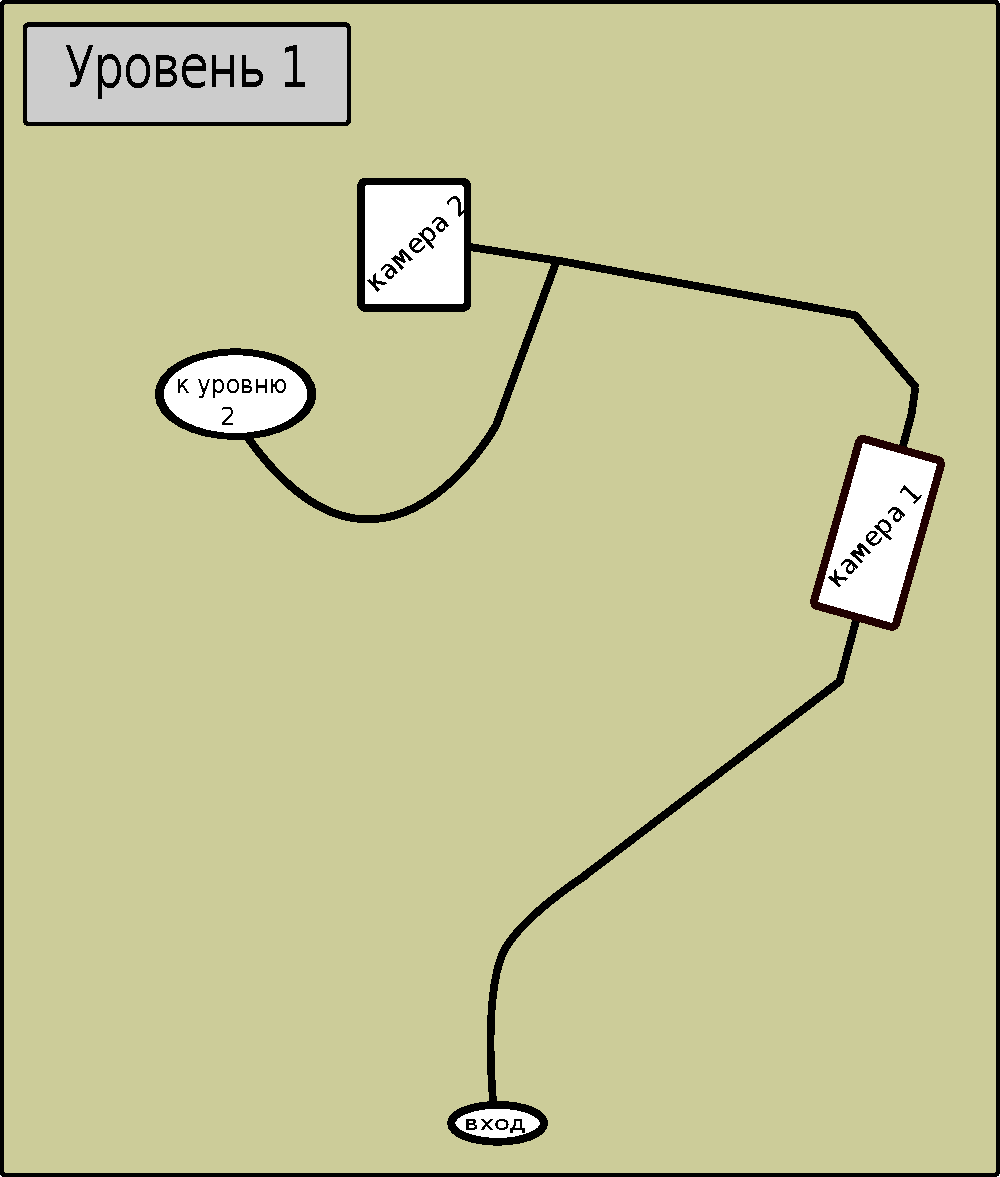
\includegraphics[width=\linewidth]{chast-zmiy/cyr-pesh/kirill-peshera-plan-level-01.pdf}
\end{center}

\vspace*{\fill}
\newpage
Камера номер 1 – проходная комната с лавками по сторонами. Высота потолка там 1,20 метра, ширина 1,40 метра. Лавки такого размера, который подошел бы карликам. 

\begin{center}
\includegraphics[width=0.96\linewidth]{chast-zmiy/cyr-pesh/\myimgprefix pesh-02.jpg}
\end{center}

\begin{center}
\includegraphics[width=0.96\linewidth]{chast-zmiy/cyr-pesh/\myimgprefix pesh-03.jpg}
\end{center}

\newpage

На плоском полу лежат бутылка и тряпка, бурый потёк – следствие недавнего дождя и нарушения былой защиты от воды. 

\vspace*{\fill}
\begin{center}
\includegraphics[width=\linewidth]{chast-zmiy/cyr-pesh/\myimgprefix pesh-05.jpg}
\end{center}
\vspace*{\fill}

\newpage

Из камеры 1 идет коридор высотой 1 метр и шириной 60 сантиметров.

\vspace*{\fill}
\begin{center}
\includegraphics[width=\linewidth]{chast-zmiy/cyr-pesh/\myimgprefix pesh-06.jpg}
\end{center}
\vspace*{\fill}

\newpage

Доходим до перекрестка около камеры 2 (она меньше «проходной комнаты» и ниже потолок).

\begin{center}
\includegraphics[width=0.92\linewidth]{chast-zmiy/cyr-pesh/\myimgprefix pesh-07.jpg}
\end{center}

Камера 2 вблизи, объектив глядит на нее и на предыдущем снимке:

\begin{center}
\includegraphics[width=0.92\linewidth]{chast-zmiy/cyr-pesh/\myimgprefix pesh-08.jpg}
\end{center}

\newpage

Замеры коридора, идущего в направлении отметки «к уровню 2». Высота 1,40 метр, ширина 75 сантиметров.

Переходим на уровень 2. Вот его план:

\begin{center}
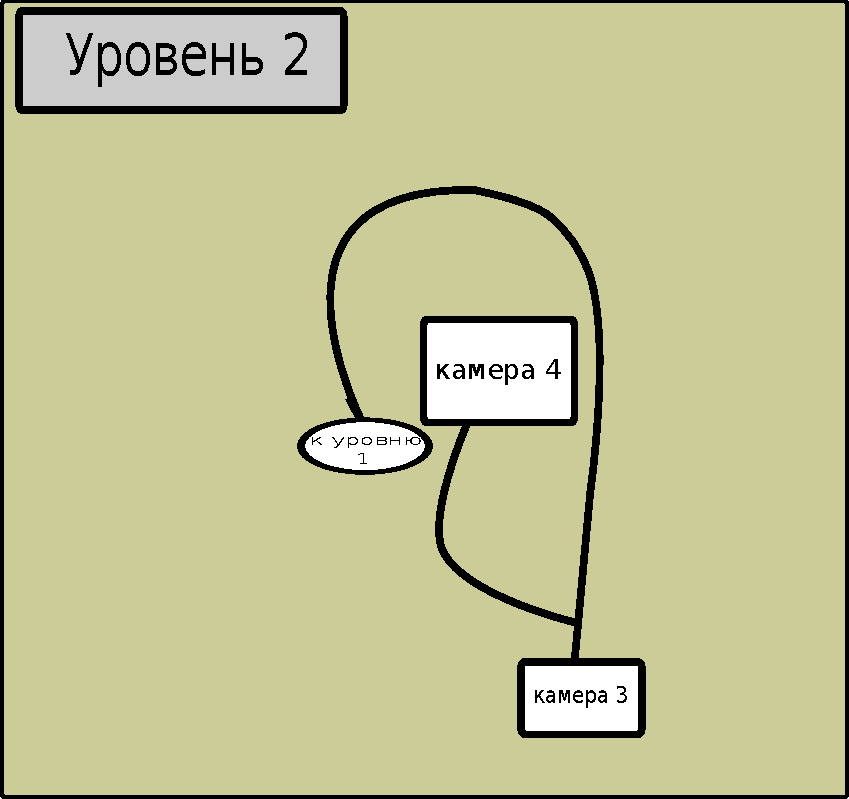
\includegraphics[width=\linewidth]{chast-zmiy/cyr-pesh/kirill-peshera-plan-level-02.pdf}
\end{center}

Когда я пишу «Уровень 2», это не значит, что вот шел себе коридор и вдруг в нем открывается яма со спуском на уровень ниже. Нет. Коридор описывает полукруг, постоянно понижаясь. В итоге вы оказываетесь в ходах, лежащих ниже, чем те, по которым пришли сюда. Прав был Антонович, говоря, что пещера формой напоминает виток спирали.

По фотографиям на следующей странице нельзя наглядно оценить высоту коридора, а число 1,40 метра звучит слишком сухо. Получится идти сильно согнувшись либо на корточках, последнее даже легче. Снова обращаю ваше внимание на ровную поверхность пола, потолка и некоторых стен.

\newpage

Это коридор, соединяющий уровень 1 и уровень 2:

\begin{center}
\includegraphics[width=\linewidth]{chast-zmiy/cyr-pesh/\myimgprefix pesh-09.jpg}
\end{center}

\begin{center}
\includegraphics[width=\linewidth]{chast-zmiy/cyr-pesh/\myimgprefix pesh-10.jpg}
\end{center}

\newpage

Затем потолок понижается, надо передвигаться только вприсядку. Не доходя до перекрестка у камеры 3, я нашел цветы – такие же, насколько знаю, есть в катакомбах Одессы и некоторых других пещерах:

\begin{center}
\includegraphics[width=0.95\linewidth]{chast-zmiy/cyr-pesh/\myimgprefix flower-01.jpg}
\end{center}

\begin{center}
\includegraphics[width=0.95\linewidth]{chast-zmiy/cyr-pesh/\myimgprefix flower-03.jpg}
\end{center}
   
\newpage

Вот впереди, внизу виден перекресток около камеры 3:

\begin{center}
\includegraphics[width=0.92\linewidth]{chast-zmiy/cyr-pesh/\myimgprefix pesh-13.jpg}
\end{center}

Камера номер 3:

\begin{center}
\includegraphics[width=0.92\linewidth]{chast-zmiy/cyr-pesh/\myimgprefix pesh-14.jpg}
\end{center}

\newpage

Перекресток около камеры 3 имеет нишу (с несколькими маленькими, пустыми подсвечниками) под стеной с надписью:

\begin{center}
\includegraphics[width=0.94\linewidth]{chast-zmiy/cyr-pesh/\myimgprefix altar-01.jpg}
\end{center}

\begin{center}
\includegraphics[width=0.94\linewidth]{chast-zmiy/cyr-pesh/\myimgprefix altar-04.jpg}
\end{center}

%\begin{center}
%\includegraphics[width=\textwidth]{/chast-zmiy/cyr-pesh/altar-06.jpg}
%\end{center}

\newpage

Также любопытен коридор к камере 4. На отрезке, примыкающем к ней, он представляет собой шкурник – лаз настолько сплюснутый, плоский, что едва можно протиснуться, между тем как ширина относительно достаточная. Вот поворот к этому шкурнику:

\begin{center}
\includegraphics[width=\textwidth]{chast-zmiy/cyr-pesh/\myimgprefix pesh-15.jpg}
\end{center}

Ширина шкурника – примерно 60 сантиметров, высота 40. Длину я не мерил, ибо полз, одновременно снимая это на видео. Там нужно именно ползти, причем подтягиваясь на руках, потому что ногами в такой тесноте особо не пошевелишь. Всё время кажется, что толща горы над тобой сейчас опустится и раздавит, хотя вот уже сколько тысяч лет прошло, а пещера жива. Впрочем, эти тысячи лет никто велосипедные трамплины над нею не устраивал и особняки рядом не строил.

%За шкурником – последняя, большая камера, я обозначил ее на карте номером 4. Она имеет длину 3,5 метра, ширину 76 сантиметров, высота – можно стоять, сгорбившись. Спустя несколько минут, проведенных здесь, дышать уже трудно от осыпающихся частиц лёсса. Пробивает на кашель.

За шкурником – последняя, большая камера, я обозначил ее на карте номером 4. Она имеет длину 3,5 метра, высота – можно стоять, сгорбившись. Спустя несколько минут, проведенных здесь, дышать уже трудно от осыпающихся частиц лёсса. Пробивает на кашель.


Кроме нескольких ниш, в этой камере находится еще одна, меньшая камера, чей пол приподнят относительно большей. Длиной она около метра, а высота такая, что я мог встать на четвереньки. На полу ее постлана ткань столь древняя, что от прикосновения обращается в прах. Кажется, что меньшая ниша представляет собой род лежанки, где поместилось бы небольшое существо размером с ребенка.

Научное исследование ткани каким-нибудь методом вроде радиоуглеродного наверняка дало бы доказательства невероятной ее древности, но это никому не надо, археологи лучше будут изучать что-то далеко от Киева, на берегу моря, там тепло и водичка рядом плещется.

Моих знаний недостаточно, чтобы по внешнему виду прийти хотя бы к поверхностным выводом, кроме того, что я столкнулся с настоящей древностью. Далее покажу фотографии. В камере за шкурником я всё снимал на видеокамеру и фотоаппарат, осознавая важность этой работы, ибо всё может быть разрушено, обвалено, разорено.

Возясь в узком пространстве, ничего толком не рассмотрел – и лишь потом, уже дома, на фотографиях заметил вещи, которых не видел на местности. Оказывается, на ткани и рядом с нею лежали два предмета, похожие на темные, красноватые свечи или охотничьи колбаски.

«Ткань» была, скорее, предметом одежды, нежели просто куском холста. Но я даже не могу судить, каким способом произведена эта ткань. Местами притрушенная сухой глиной, частью она распалась в темные волокнистые ошметки. Но сделаем важный вывод! Сначала – повторюсь, малейшее касание обращает эту ткань в прах. А это значит, ткань не трогали долгие годы! Никто не лежал в этой нише может быть целые века! Странно, ведь остальная часть пещеры достаточно истоптана любителями.

Да, в последней камере валяется пакет невесть с чем твердым, да в углу торчит вкопанная пластиковая бутылка, но нишу с лежанкой щадили, по время моего посещения пещеры осенью 2013 года.
 
Вообще камера номер 4 – самое безопасное место в пещере, поскольку для обороны надо будет держать только сплюснутый шкурник. Всякого, кто через него полезет, остановить весьма просто – а вот тот, кто продвигается по шкурнику, лишен возможности как-либо нападать.

Приступим же к осмотру последней камеры. На первом снимке лежанки не видно, это другие ниши. 

\begin{center}
\includegraphics[width=\linewidth]{chast-zmiy/cyr-pesh/\myimgprefix IMG_2814.JPG}
\end{center}

\newpage

Здесь я повернул объектив фотоаппарата чуть левее, а нахожусь спиной к лежанке. На полу – моя MiniDV-видеокамера:
\vspace*{\fill}
\begin{center}
\includegraphics[width=\linewidth]{chast-zmiy/cyr-pesh/\myimgprefix IMG_2815.JPG}
\end{center}
\vspace*{\fill}
\newpage

Стены, потолок:

\begin{center}
\includegraphics[width=\linewidth]{chast-zmiy/cyr-pesh/\myimgprefix IMG_2816.JPG}
\end{center}

\begin{center}
\includegraphics[width=\linewidth]{chast-zmiy/cyr-pesh/\myimgprefix IMG_2813.JPG}
\end{center}

\newpage

Вид на нишу с лежанкой:

\begin{center}
\includegraphics[width=\linewidth]{chast-zmiy/cyr-pesh/\myimgprefix IMG_2832.JPG}
\end{center}

\begin{center}
\includegraphics[width=\linewidth]{chast-zmiy/cyr-pesh/\myimgprefix IMG_2812.JPG}
\end{center}

\newpage

В тупике ниши с лежанкой – еще одна нишка в стене:

\begin{center}
\includegraphics[width=0.98\linewidth]{chast-zmiy/cyr-pesh/\myimgprefix IMG_2817.JPG}
\end{center}

Стена над лежанкой:

\begin{center}
\includegraphics[width=0.98\linewidth]{chast-zmiy/cyr-pesh/\myimgprefix IMG_2818.JPG}
\end{center}

\newpage

Ткань в нише-лежанке:

\begin{center}
\includegraphics[width=\linewidth]{chast-zmiy/cyr-pesh/IMG_2820.JPG}
\end{center}

\begin{center}
\includegraphics[width=\linewidth]{chast-zmiy/cyr-pesh/IMG_2819.JPG}
\end{center}

\newpage

Надписи над лежанкой:

\begin{center}
\includegraphics[width=0.98\linewidth]{chast-zmiy/cyr-pesh/\myimgprefix IMG_2829.JPG}
\end{center}

Потолок:

\begin{center}
\includegraphics[width=0.98\linewidth]{chast-zmiy/cyr-pesh/\myimgprefix IMG_2811.JPG}
\end{center}

\newpage

Вид на шкурник со стороны камеры 4:

\begin{center}
\includegraphics[width=\linewidth]{chast-zmiy/cyr-pesh/\myimgprefix IMG_2833.JPG}
\end{center}

\begin{center}
\includegraphics[width=\linewidth]{chast-zmiy/cyr-pesh/\myimgprefix IMG_2834.JPG}
\end{center}

\newpage

Стены пещеры покрыты надписями, черточками, символами. Если не указан год, сложно отличить современное от старого или даже древнего. Различимы несколько надписей за тридцатые-сороковые годы 20 века. В одном месте, в нише над лавкой, написаны три строки, верхняя из которых плохо читается и содержит имя «АЛЁША», ниже идет «1945», еще ниже: «умер», и под этим цифры, будто «1 5 4». К сожалению, я не помню, в каких именно частях пещеры какие снимки с надписями сделаны, кроме упомянутых ранее, поэтому приведу их в случайном порядке.

Эти стенные надписи должны цениться на вес золота и быть исследованы и расшифрованы. Среди новейших наносов обнаружится первобытное, а пещера раскроет часть своих тайн и задаст новые загадки.

Надо много сил и свободного времени, чтобы, поскольку никто не делает из пещеры настоящий заповедник, тщательно сфотографировать все граффити и потом основательно их изучить. 

\vspace*{\fill}
\begin{center}
\includegraphics[width=\linewidth]{chast-zmiy/cyr-pesh/\myimgprefix nadpis-01.jpg}
\end{center}
\vspace*{\fill}

\newpage

\vspace*{\fill}
\begin{center}
\includegraphics[width=\linewidth]{chast-zmiy/cyr-pesh/\myimgprefix nadpis-03.jpg}
\end{center}

\begin{center}
\includegraphics[width=\textwidth]{chast-zmiy/cyr-pesh/\myimgprefix nadpis-04.jpg}
\end{center}
\vspace*{\fill}

\newpage

\vspace*{\fill}
\begin{center}
\includegraphics[width=\textwidth]{chast-zmiy/cyr-pesh/\myimgprefix nadpis-05.jpg}
\end{center}

\begin{center}
\includegraphics[width=\textwidth]{chast-zmiy/cyr-pesh/\myimgprefix IMG_2805.JPG}
\end{center}
\vspace*{\fill}

\newpage

\vspace*{\fill}
\begin{center}
\includegraphics[width=\textwidth]{chast-zmiy/cyr-pesh/\myimgprefix nadpis-02.jpg}
\end{center}

\begin{center}
\includegraphics[width=\textwidth]{chast-zmiy/cyr-pesh/\myimgprefix nadpis-06.jpg}
\end{center}
\vspace*{\fill}

\newpage
\vspace*{\fill}
\begin{center}
\includegraphics[width=\textwidth]{chast-zmiy/cyr-pesh/\myimgprefix nadpis-07.jpg}
\end{center}

\begin{center}
\includegraphics[width=\textwidth]{chast-zmiy/cyr-pesh/\myimgprefix IMG_20130714_172356.jpg}
\end{center}
\vspace*{\fill}

\newpage


\vspace*{\fill}
\begin{center}
\includegraphics[width=\textwidth]{chast-zmiy/cyr-pesh/\myimgprefix IMG_20130714_172436.jpg}
\end{center}

\begin{center}
\includegraphics[width=\textwidth]{chast-zmiy/cyr-pesh/\myimgprefix IMG_20130714_172530.jpg}
\end{center}
\vspace*{\fill}

\newpage

Еще снимки.

В некоторых местах потолок пещеры покрыт копотью:
\vspace*{\fill}

\begin{center}
\includegraphics[width=\textwidth]{chast-zmiy/cyr-pesh/\myimgprefix IMG_2708.JPG}
\end{center}
\vspace*{\fill}

\newpage

Обвалившиеся глыбы лёсса на переднем плане и справа красноречиво говорят о том, что трамплин над пещерой разрушает её.
\vspace*{\fill}

\begin{center}
\includegraphics[width=\textwidth]{chast-zmiy/cyr-pesh/\myimgprefix IMG_2798.JPG}
\end{center}
\vspace*{\fill}

\newpage

Один из коридоров. Четко видно его закругление.
\vspace*{\fill}

\begin{center}
\includegraphics[width=\textwidth]{chast-zmiy/cyr-pesh/\myimgprefix IMG_2799.JPG}
\end{center}
\vspace*{\fill}

\newpage

Перекресток около камеры 2:
\vspace*{\fill}

\begin{center}
\includegraphics[width=\textwidth]{chast-zmiy/cyr-pesh/\myimgprefix IMG_2800.JPG}
\end{center}
\vspace*{\fill}

\newpage

Снова коридор. На полу – потёк от ливня, прошедшего на поверхности. Без первоначального, опущенного козырька над входом, в пещеру далеко попадает вода.
\vspace*{\fill}

\begin{center}
\includegraphics[width=\textwidth]{chast-zmiy/cyr-pesh/\myimgprefix IMG_2801.JPG}
\end{center}
\vspace*{\fill}

\newpage

Неясно, когда в стене была сделана эта ниша, однако надписи в копоти вполне современные:
\vspace*{\fill}

\begin{center}
\includegraphics[width=\textwidth]{chast-zmiy/cyr-pesh/\myimgprefix IMG_2802.JPG}
\end{center}
\vspace*{\fill}

\newpage

Еще одна ниша с углублениями непонятного назначения:

\begin{center}
\includegraphics[width=\textwidth]{chast-zmiy/cyr-pesh/\myimgprefix nadpis-08.jpg}
\end{center}

Таково Логово Змиево, пещера, которой пользуются уже несколько тысяч лет. Цивилизация подобралась сюда вплотную и ничего хорошего от этого ждать не следует.

Время течет в ней, кажется, иначе, чем снаружи – однако ничем это доказать я не могу. Когда был внутри, снимая камеру за шкурником, то полагал, что пробыл под землей около получаса максимум, а выбравшись наружу, узнал от ожидавшего там Коли, что прошло пятьдесят минут.

Вылезаешь – болят под коленями мышцы, ведь в пещере надо передвигаться на карачках либо сильно пригнувшись. В местах с особо низким потолком вполне можно ободрать об него спину. Звуки слышатся глухо, скрадываются. Отойдешь метров пятнадцать от входа, и уже не слышно, что тебе кричат оттуда, с бела света. Мобильная связь, конечно же, не работает.

В пещере удивляют многие вещи. О миниатюрных размерах я уже говорил. Христианские монахи рыли себе пещеры просторнее. И у них другая структура пещер, а тут всё подчинено неуловимой для меня функциональности. Как отсеки на подводной лодке. Естественная вентиляция, четкие очертания стен, плоские пол и потолок – проведена огромная работа! Ходы этой пещеры не рылись по случайному вдохновению. Пещера слишком продумана. Вначале был проект. Потом – его воплощение.

Теперь задумаемся. Антонович писал, что обнаружил в «передней пещере» стоянку людей каменного века. 

Передняя пещера – это теперь открытая площадка перед входом. Антонович говорит, что первобытные люди, оставившие на память кучу мусора, лепили без помощи гончарного круга нехитрую посуду, пользовались кремневыми орудиями. Кроме того, в статье ученый упоминает «очаг, нарочито сложенный из глыб валуна». Антонович нашел в мусоре также, в малом количестве, остатки костей диких быка, свиньи, лошади.

Это первобытные охотники и собиратели ракушек выкопали такое сложное архитектурное сооружение? 

Нет. Они просто посещали его предбанник. Можно возразить, что вначале был «предбанник», а в позднейшее время его продолжили. Но предбанник сам по себе был частью большого плана. Я уже говорил об устройстве «передней пещеры» Антоновича – она двускатная.

Раньше я не знал о сообщениях Роговича и Бобровского о лестничных уступах на склоне. И поныне не знаю, к чему они вели – к Змиевой пещере или к другому месту? 

Если к Змиевой, то вопрос попадания туда снизу вверх пожалуй отбросим, иначе же остается предположить, что к пещере подлетали либо карабкались по каким-то веревочным лестницам или канатам. Повторюсь – при исследовании местности я не заметил около пещеры явных, упомянутых уступов. Возможно, они были раньше. Либо находятся в стороне и от них остались те укрепленные участки горы, про которые я писал.

Но если ступеней всё же не было под пещерой, то что нужно дикому человеку сделать, дабы вырыть хотя бы вход в пещеру? 

Надо каким-то макаром закрепиться на почти отвесном склоне, на большой высоте, и при помощи какой-нибудь твердой палки рыть нору под углом вверх и вглубь, держась в лучшем случае за торчащие из склона корешки.

При этом дикий человек, в любом случае, заранее должен держать в уме проект двускатного подземного хода, иначе зачем ему невероятно усложнять себе жизнь и копать снизу вверх, когда проще сверху вниз? Итак, даже предбанник – плод раздумий, затем воплощения.

Был ли способен на такое первобытный человек, чей «мусор» нашел Антонович? Был ли это вообще человек, а не другое существо, более развитое, но с – по какой-то причине – примитивным набором орудий? Как выброшенные после кораблекрушения сбивают палками кокосы, а вместо веревок используют лианы.

%Вопрос. А как же залезать в пещеру, если вход расположен снизу вверх, да еще на большой высоте? Ответ, если не выдумывать канатных лестниц или веревок, очевиден – только подлететь.

%Теперь отложим в сторону задачу о том, что было раньше – только предбанник, или предбанник вместе с пещерой, и как туда добирались в былое время. 

Тимур Бобровский в газетном интервью сообщил, что нашел «сразу при входе» (значит, близко и к находке Антоновича) сосуд трипольской культуры, эпохи энеолита – это четвертое-третье тысячелетие до нашей эры. А свои находки керамики Антонович описывал, как «плохо вылепленные и едва обожженные». 

Полагаю, что между качественной трипольской керамикой, хоть тоже не знавшей гончарного круга, и плохонькими горшками Антоновича прошло немало времени. Сколько? Несколько сотен или тысяч лет?

Но выходит, на протяжении всего этого времени около входа в пещеру бывали разумные существа, пользующиеся предметами. По крайней мере делаем вывод, что передняя часть пещеры использовалась непрерывно на протяжении периода времени, превышающего срок жизни человека. Должно было смениться много поколений людей!

А после «трипольцев»? Я видел на стенах пещеры надписи, однозначно относящиеся к сороковым годам 20 века. И по сей день. Это значит, что с сороковых годов уже саму пещеру посещают непрерывно. Бобровский писал о граффити 1743 года, не приведя однако его содержание.

Во временном промежутке от «трипольцев» до 1940-х – кто точно был в пещере? Антонович был. Переднюю площадку он описал, а вот что внутри пещеры – нет. Почему? Был в пещере, подсчитал длину, узнал, что спиралью идет, так хоть пару слов черкни, что видел. Полное молчание. Состояние коридоров, может какие-то предметы... Нет, куча «мусора» перед входом, и ни слова о том, что за входом.

Даже без мысли о том, что это – Логово Змия, Кирилловская пещера – явление странное. Сложное, огромное подземное сооружение, не относящееся к христианству.

А как насчет летописного выражения о поганском населении местности, где братья заложили город Киев – «бяху же погани, жряху идолом в колодезем». То есть приносили жертвы идолам в колодезях. А если колодези здесь не водные криницы, а пещеры, ходы под землю? У Даля читаем одно из значений слова «колодезь»: «узкая и глубокая яма; рудная дудка, спуск в землю». 

%Буквально летопись говорит, что язычники приносили жертвы существам, обитавшим в пещерах! 

Вспомним и предание, что Змей обложил Киев живой данью. В былинах же, когда Владимир, позже по времени, крестил Русь, выплата дани вероятно прекратилась, поэтому Змеи начали совершать на Киев налёты. Мол, не хотите давать – сами возьмем.

Что, если именно такой Змей, небольшого роста, оснащенный устройством для полета, и возможно пулевым оружием и огнеметом («громом и молнией») – назывался Перуном, а в былинах христианского времени – Змеем, Змеем Горынычем?

Богатыри же одни имели возможности, быть может технические, со Змеями сражаться. Хотя языковеды говорят нам о сходстве слов богатырь и «батыр», я предположу, что «богатырь» это существительное от глагола «богати», означающего служение христианскому богу. Что указывало на религиозную принадлежность таких воинов.

Пещеры Смородинского спуска каким-то образом использовались Змеями.

Позже, вероятно, пещеры эти, по крайней мере Змиева, веками слыли священными, на что указывают следы древнего «мусора» в предбаннике пещеры, а не внутри.

Принятое Антоновичем за стоянку, было, полагаю, местом жертвоприношений – люди приносили туда что имели или что требовалось – однако не жили ни в предбаннике, ни внутри, иначе бы с чего им ограничивать себя только предбанником? А раз ограничивали, значит, внутрь пещеры их не впускал страх перед священным либо жрец. Допускаю, что само существо, одно из тех, кому поклонялись, лежало на описанном мною лежаке с тканью. Идол в колодезе, змий. И камера за шкурником была его усыпальницей.

%Сведения удалось собрать лишь о Кирилловской. 

%Если пройти от нее дальше по краю склона, в сторону улицы Фрунзе, будет несколько загадочных провалов в земле, возможно это следы былых подземелий. Теперь они превращены в свалки.

%А ведь такой древности, как эта пещера, даже без Змеев, нет больше ни в одном городе. В Киеве есть, однако никому не нужная. Гадят у входа, рисуют на стенах поверх старинных граффити, прыгают над пещерой с трамплина, строят неподалеку терема! Ничего не нужно, ни прошлого, ни будущего, только бы овладеть настоящим.
